
\begin{figure}
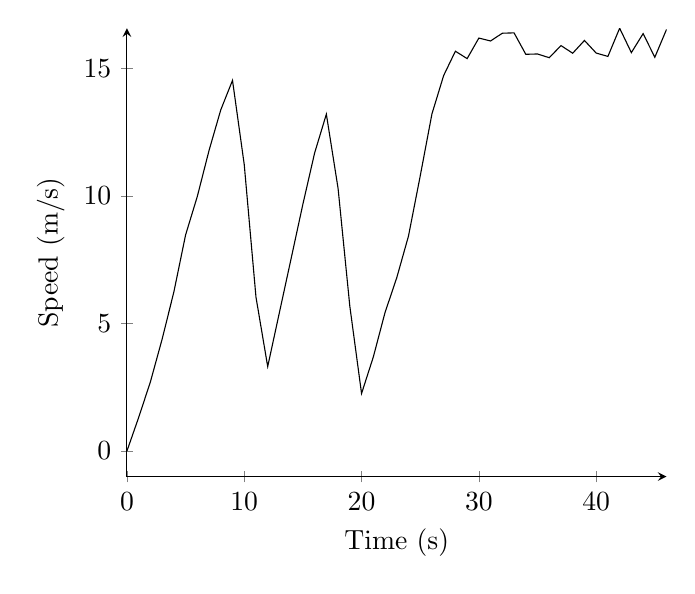
\begin{tikzpicture}
\begin{axis}[
legend style={anchor=west},
axis x line=bottom,
axis y line=left,
ymin=-1,
xlabel=Time (s),
ylabel=Speed (m/s),
]
\addplot[] coordinates {
(0, 0.0)
(1, 1.31607864721)
(2, 2.7125904517)
(3, 4.38742730126)
(4, 6.23739365721)
(5, 8.47480058612)
(6, 9.98592031043)
(7, 11.7896095538)
(8, 13.3818055855)
(9, 14.5357318723)
(10, 11.2348986996)
(11, 6.03781964588)
(12, 3.31344123948)
(13, 5.4385047626)
(14, 7.55715051189)
(15, 9.68280471356)
(16, 11.6906111864)
(17, 13.2117582583)
(18, 10.2966178112)
(19, 5.68136058183)
(20, 2.25637514077)
(21, 3.68513844607)
(22, 5.43086649404)
(23, 6.79566539349)
(24, 8.43078448806)
(25, 10.7861941406)
(26, 13.2221087155)
(27, 14.7294732686)
(28, 15.6805743533)
(29, 15.3907576893)
(30, 16.197267971)
(31, 16.0822139756)
(32, 16.3864503725)
(33, 16.4003498075)
(34, 15.5598241658)
(35, 15.5722923446)
(36, 15.4257489339)
(37, 15.9013664891)
(38, 15.6014995707)
(39, 16.102691495)
(40, 15.608437694)
(41, 15.4763429591)
(42, 16.5823435477)
(43, 15.6260336333)
(44, 16.3699291309)
(45, 15.4448962045)
(46, 16.5384550445)
};

\end{axis}
\end{tikzpicture}
\label{tik:0:19}
\caption{0 percent diving with GSC on route $19$}
\end{figure}
